% Fichier  : projet.tex
% Format   : LaTeX file
% Auteur   : Florent Hivert
% A propos : Master 2 / Combinatoire
% Date     : lun. oct.  2 14:09:41 CEST 2017
%%%%%%%%%%%%%%%%%%%%%%%%%%%%%%%%%%%%%%%%%%%%%%%%%%%%%%%%%%%%%%%%%%%%%%%%%%%%%%%
\documentclass[11pt]{article}

\usepackage[svgnames]{xcolor}
\usepackage{styles/tdtp,array,amsmath}
\usepackage[T1]{fontenc}
\usepackage[utf8]{inputenc}
\usepackage[francais]{babel}
\usepackage{multicol}
\usepackage{styles/tikz-uml}
\usepackage{hyperref}
\usepackage{listingsutf8}


\lstset{inputencoding=utf8/latin1,
  language=python,
%  numbers=left,
  lineskip=-.2ex,
  basicstyle={\ttfamily},
  columns=fixed,
  fontadjust=true,
  basewidth={1.09ex},
  showspaces=false, showstringspaces=false,
  commentstyle=\color{DarkGreen},
  keywordstyle=\color{DarkBlue},
  stringstyle=\color{DarkBlue},
}

\newcommand\todo[1]{\textcolor{red}{ToDo: #1}}

\usetikzlibrary{positioning}
%
%\CORRECTIONtrue
\projet{de Combinatoire}
\course{Master d'informatique}
\group{Génération Combinatoire}
\theme{Génération d'objets combinatoires décrit par une grammaire}
%
\newcommand{\cpl}[1]{\overline{#1}}
\renewcommand{\emph}[1]{\textbf{#1}}
\newcounter{asuivre}
\newenvironment{ask}{\begin{enumerate}}%
                       {\setcounter{asuivre}{\theenumi}\end{enumerate}}
\newenvironment{asks}{\begin{enumerate}\setcounter{enumi}{\theasuivre}}%
                       {\setcounter{asuivre}{\theenumi}\end{enumerate}}


\newcommand{\Python}{\texttt{Python}}

\begin{document}
\maketitle

\begin{abstract}
  Le but de ce projet est de compter et d'engendrer l'ensemble des objets
  combinatoires étiqueté décrits par une grammaire. Il est ainsi possible
  d'engendrer une grande variété d'objets comme des ensembles, des arbres ou
  des mots.  \smallskip

  Le projet sera implanté en \Python{}. On pourra travailler seul ou en
  binôme. La date de remise sera précisée ultérieurement. Toutes les fonctions
  de ce projet devront être commentées et testées.

  On rédigera également un \textbf{rapport} présentant les fonctionnalités et
  répondant aux questions théoriques du sujet. Les algorithmes et choix
  d'implantations devront être expliqués. 
\end{abstract}

\section{Grammaires étiquetées : Introduction et quelques exemples}
%%%%%%%%%%%%%%%%%%

\subsection{Objets étiquetés}


Dans ce projet, nous allons construire et implémenter des grammaires pour
décrire des objets \textbf{étiquetés}. Par rapport à ce que l'on a vu en
cours, on ne parlera pas de l'ensemble des objets de taille $n$, mais de
\textbf{l'ensemble des objets étiquetés par les éléments de $S$}. L'ensemble
des étiquettes $S$ sera décrit par une \textbf{liste supposée triée et sans
  doublons}. Un objet décrit par la grammaire devra contenir \textbf{toutes
  les étiquettes une fois et une seule}. Avant de décrire les grammaires nous
commençons par quelques exemples.

\subsubsection{Séquences}
\label{seq:sequences}

\begin{enumerate}
\item Séquences simples : les objets de ce type sont les listes contenants
  toutes les étiquettes. Ce sont donc les permutations de l'entrée $S$. Ainsi
\begin{verbatim}
Seq.list([1,2,3]) = [[1,2,3],[1,3,2],[2,1,3],[2,3,1],[3,1,2],[3,2,1]
\end{verbatim}
\item Séquence ordonnées : les objets de ce type sont les listes contenants
  toutes les étiquettes dans l'ordre. Il n'y a donc qu'un seul objet: la liste
  donnée en entrée:
\begin{verbatim}
SortedSeq.list([1,2,3]) = [[1,2,3]]
\end{verbatim}
\item Séquence cyclique : les objets de ce type sont les listes à permutation
  cyclique prêt. On peut donc supposer que le plus petit élément est au début:
\begin{verbatim}
Cycle.list([1,2,3]) = [[1,2,3],[1,3,2]]
Cycle.list([0,1,2,3]) =
        [[0,1,2,3],[0,1,3,2],[0,2,1,3],[0,2,3,1],[0,3,1,2],[0,3,2,1]
\end{verbatim}
\item Séquence zig-zag : les objets de ce type sont les listes
  $(a_0<a_1>a_2<a_3>a_4<\dots)$:
\begin{verbatim}
ZigZag.list([1,2,3]) = [[1,3,2],[2,3,1]]
ZigZag.list([1,2,3,4]) =
        [[1,3,2,4],[1,4,2,3],[2,3,1,4],[2,4,1,3],[3,4,1,2]]
\end{verbatim}
\end{enumerate}

\subsubsection{Partitions d'ensemble}
\label{seq:set-partitions}

Pour un ensemble $S$ donné, les \emph{partitions d'ensemble} sont toutes
les façons de découper $S$ en sous ensemble.

Par exemple, il y a 5 façons de partitionner l'ensemble $\lbrace 1,2,3 \rbrace$ :

\begin{itemize}
\item $\lbrace\lbrace 1 \rbrace, \lbrace 2 \rbrace, \lbrace 3 \rbrace\rbrace$
\item $\lbrace\lbrace 1,2 \rbrace, \lbrace 3 \rbrace\rbrace$,
\item $\lbrace\lbrace 1,3 \rbrace, \lbrace 2 \rbrace\rbrace$,
\item $\lbrace\lbrace 1 \rbrace, \lbrace 2,3 \rbrace\rbrace$,
\item $\lbrace\lbrace 1,2,3 \rbrace\rbrace$
\end{itemize}

\subsubsection{Arbres binaires}
\label{seq:binary-trees}

Les grammaires étiquetées permettent non seulement d'obtenir des séquences de nombre
mais aussi des objets plus complexes tels que les arbres binaires.

Il y a deux façons classiques d'étiqueter les arbres binaires :
\begin{itemize}
\item étiquetage des feuilles;
\item étiquetage des noeuds internes.
\end{itemize}

Dans le fichier {\tt LabelledBinaryTree.py} vous trouverez une classe python très proche
de celle vue en TP qui permet de représenter des arbres binaires étiquetés (sur les noeuds
ou les feuilles).

Par exemple, on peut créer les arbres suivants:

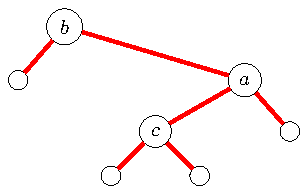
\includegraphics[scale=.5]{images/arbre_etiquete1.pdf}

\begin{verbatim}
>>> t = Node(Leaf(), Node(Node(Leaf(),Leaf(),"c"), Leaf(), "a"), "b")
>>> t
b(leaf, a(c(leaf, leaf), leaf))
\end{verbatim}

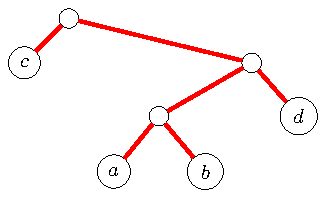
\includegraphics[scale=.5]{images/arbre_etiquete2.pdf}

\begin{verbatim}
>>> t = Node(Leaf("c"), Node(Node(Leaf("a"),Leaf("b")), Leaf("d")))
>>> t
>>> (c, ((a, b), d))
\end{verbatim}

Les grammaires étiquetées nous permettront par exemple d'engendrer :

\begin{itemize}
\item L'ensemble des arbres dont les noeuds sont étiquetés par un ensemble donné.
\item L'ensemble des arbres dont les feuilles sont étiquetées par un ensemble donné.
\item Les arbres croissants : l'ensemble des arbres dont les noeuds sont étiquetés par 
un ensemble ordonné donné tels que l'étiquette d'un noeud soit toujours inférieure 
aux étiquettes de ses fils.
\item Les arbres binaires de recherche : l'ensemble des arbres dont les noeuds sont étiquetés par 
un ensemble ordonné donné tels que l'étiquette d'un noeud soit toujours supérieure
à toutes les étiquettes de son fils gauche et inférieure à toutes les étiquettes
de son fils droit.
\end{itemize}

\begin{tabular}{l|l}
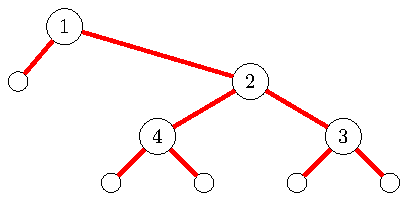
\includegraphics[scale=.5]{images/arbre_croissant.pdf} & 
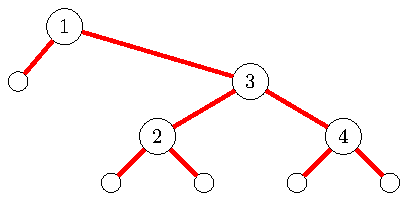
\includegraphics[scale=.5]{images/abr.pdf} \\
Exemple arbre croissant & Exemple ABR
\end{tabular}

\subsection{Définitions formelles des grammaires étiquetées}
%%%%%%%%%%%%%%%%%%%%%%%%%%%%%%%%%%%%%%

Une grammaire décrit récursivement un ensemble d'objets. Elle est constituée
d'un ensemble de règles ayant chacune un nom (chaîne de caractères). Le nom
d'une règle est appelé \emph{symbole non-terminal} ou plus simplement
non-terminal de la grammaire.  \medskip

Une \emph{règle de grammaire} $R$ décrit un ensemble qui est
\begin{itemize}
\item soit un singleton dont le seul élément est un objet
  \emph{atomique} construit en utilisant une seule étiquette.
\item soit un ensemble dont le seul élément est un objet
  \emph{vide} sans étiquette (par exemple la chaîne vide ou l'arbre vide).
\item soit l'\emph{union de deux ensembles} décrit par deux
  non-terminaux $N_1$ et $N_2$;
\item soit une variante du \emph{produit
    cartésien de deux ensembles}\footnote{les variantes possibles sont décrites un peu plus tard} 
    décrit par deux non-terminaux $N_1$ et $N_2$;
  L'ensemble est alors construit à partir des paires d'éléments $(e_1, e_2)
  \in N_1 \times N_2$.
\end{itemize}
\medskip

La \emph{taille} ou \emph{poids} d'un objet est le nombre d'étiquette qu'il
contient. Le poids d'un élément correspondant à une paire $(e_1, e_2)$ est
donc la somme des poids de $e_1$ et de $e_2$.

À chaque non-terminal on associe la taille du plus petit objet qui en dérive.
Cette taille est appelé \emph{valuation} du non-terminal.

Le but du projet est de permettre à un utilisateur de décrire une grammaire
en python sous la forme d'un dictionnaire associant une règle à chaque 
non-terminal et calculant : 
\begin{itemize}
\item Le nombre d'objet d'une certaine taille décrits par la grammaire (méthode {\tt count})
\item La liste des objets étiquetés par une liste d'étiquettes donnée (méthode {\tt list})
\item Un objet identifié par son rang dans la liste (méthode {\tt unrank})
\item Le rang d'un objet donné (méthode {\tt rank})
\end{itemize}

\subsection{Quelques exemples de base (mais indispensables !)}

Commençons par des exemples triviaux de grammaires. Nous vous présentons 
à chaque fois la description de la grammaire et son implantation python telle
qu'elle devra fonctionner lorsque vous aurez réalisé le projet. 

Tout le code python de déclaration des grammaires avec les tests associés se trouve
dans le fichier {\tt tests.py}.

\subsubsection{La Grammaire singleton}

Voici une grammaire contenant une unique règle de type {\tt Singleton}. Cette 
grammaire ne peut engendrer que des objets de taille 1. 

\begin{tabular}{lll}
\textbf{Singl} & $\rightarrow$ & Singleton
\end{tabular}

En python, on l'implantera de cette façon :

\lstinputlisting[firstline=10,lastline=12]{code/tests.py}

Ici, l'argument {\tt lambda x:x} est donné pour initialiser l'objet {\tt SingletonRule}.
Cela correspond à la fonction qui sera utilisée pour concrètement fabriquer l'objet 
combinatoire associé à une étiquette. Dans le cas de cette grammaire, c'est une fonction triviale qui prend l'étiquette
(typiquement une chaîne de caractère ou un entier) en argument et la renvoie directement. 
On verra dans certains cas que cette fonction peut être plus complexe, par exemple dans le
cas des arbres binaires.

Voilà quelques exemples d'utilisation de cette grammaire et des résultats attendus pour les méthodes 
{\tt count} et {\tt list} que vous devrez implanter. La description précise de ces méthodes et des 
algorithmes associés est donnée en Section~\ref{seq:algo}.

\lstinputlisting[firstline=14,lastline=24]{code/tests.py}

\subsubsection{La Grammaire Epsilon}

Voici une grammaire contenant une unique règle de type {\tt Epsilon}. Cette 
grammaire n'engendre qu'un objet unique de taille 0. Dans l'exemple suivant
c'est la chaîne vide.

\begin{tabular}{lll}
\textbf{Empty} & $\rightarrow$ & Epsilon(mot vide)
\end{tabular}

En python, on l'implantera de cette façon :

\lstinputlisting[firstline=28,lastline=30]{code/tests.py}

L'objet {\tt Epsilon} prend en paramètre l'objet de taille 0 qu'il crée. Voilà quelques exemples 
d'utilisation de cette grammaire et des résultats attendus pour les méthodes 
{\tt count} et {\tt list} que vous devrez implanter.

\lstinputlisting[firstline=32,lastline=42]{code/tests.py}

\subsubsection{Les permutations de taille 2}

Voilà un premier exemple de grammaire à 2 règles qui engendre les permutations de taille~2.

\begin{tabular}{lll}
\textbf{Perms} & $\rightarrow$ & Produit(\textbf{Letter}, \textbf{Letter}) \\
\textbf{Letter} & $\rightarrow$ & Singleton
\end{tabular}

En python, on l'implantera de cette façon :

\lstinputlisting[firstline=48,lastline=51]{code/tests.py}

Remarquez que l'objet {\tt ProductRule} prend en paramètre une fonction qui fabrique un
objet combinatoire à partir de deux objets donnés. Voilà quelques exemples 
d'utilisation de cette grammaire et des méthodes {\tt count} et {\tt list} que vous devrez implanter.

\lstinputlisting[firstline=53,lastline=64]{code/tests.py}

\subsubsection{Les permutations de toute taille}

Voilà le premier exemple de grammaire intéressante, c'est-à-dire qui engendre
une famille d'objet quelle que soit la taille. Cela nécessite une définition récursive.

\begin{tabular}{lll}
\textbf{Perms} & $\rightarrow$ & Union(\textbf{Empty}, \textbf{NonEmpty}) \\
\textbf{NonEmpty} & $\rightarrow$ & Product(\textbf{Letter}, \textbf{Perms}) \\
\textbf{Empty} & $\rightarrow$ & Epsilon(permutation vide) \\
\textbf{Letter} & $\rightarrow$ & Singleton
\end{tabular}

En python, on l'implantera de cette façon :

\lstinputlisting[firstline=68,lastline=90]{code/tests.py}

\subsubsection{Arbres binaires}

Voici pour commencer la grammaire qui engendre les arbres binaires
dont les \textbf{feuilles} sont étiquetées.

\begin{tabular}{lll}
\textbf{Tree} & $\rightarrow$ & Union(\textbf{Node}, \textbf{Leaf}) \\
\textbf{Node} & $\rightarrow$ & Product(\textbf{Tree}, \textbf{Tree}) \\
\textbf{Leaf} & $\rightarrow$ & Singleton
\end{tabular}

Ce qui en python, s'implante par

\lstinputlisting[firstline=148,lastline=152]{code/tests.py}

Remarquez que les objets {\tt Singleton} et {\tt ProductRule} prennent 
directement les fonctions {\tt Leaf} et {\tt Node} en paramètre pour
la création des objets. Voilà les résultats attendus. Notez que
la taille de l'arbre est ici le nombre de feuilles.

\lstinputlisting[firstline=156,lastline=165]{code/tests.py}

Voici l'implantation  d'une grammaire pour implanter les arbres dont les noeuds internes 
sont étiquetés. Cette fois la taille de l'arbre est donnée par le nombre
de noeuds internes et les feuilles sont dont de taille 0.

\lstinputlisting[firstline=169,lastline=185]{code/tests.py}


\subsection{Les différents produits}
\label{seq:product}

Pour que l'on obtienne un comportement intéressant avec les étiquettes, il
faut pouvoir contrôler la leurs provenance. On va donc distinguer trois
produits.
\begin{enumerate}
\item le \textbf{produit cartésien ordinaire} noté \texttt{Product}. Les
  étiquettes se répartissent alors de toutes les manières possibles. Ainsi,
  la règle \textbf{C} $\rightarrow$ Product(\textbf{A}, \textbf{B})
  sur les étiquettes $[1,2,3]$ engendre l'union des ensembles suivant
\begin{align*}
&\textbf{A}([]) \times \textbf{B}([1,2,3]) \\
 &\textbf{A}([1]) \times \textbf{B}([2,3]) \\ 
 &\textbf{A}([2]) \times \textbf{B}([1,3]) \\ 
 &\textbf{A}([3]) \times \textbf{B}([1,2]) \\ 
 &\textbf{A}([1,2]) \times \textbf{B}([3]) \\ 
 &\textbf{A}([1,3]) \times \textbf{B}([2]) \\ 
 &\textbf{A}([2,3]) \times \textbf{B}([1]) \\ 
 &\textbf{A}([1,2,3]) \times \textbf{B}([])
\end{align*}

\item le \textbf{produit cartésien boxed} noté \texttt{BoxProduct}. 
L'ensemble gauche contient forcément la plus petite étiquette.
Ainsi, la règle \textbf{C} $\rightarrow$ BoxProduct(\textbf{A}, \textbf{B})
  sur les étiquettes $[1,2,3]$ engendre l'union des ensembles suivant
\begin{align*}
 &\textbf{A}([1]) \times \textbf{B}([2,3]) \\ 
 &\textbf{A}([1,2]) \times \textbf{B}([3]) \\ 
 &\textbf{A}([1,3]) \times \textbf{B}([2]) \\ 
 &\textbf{A}([1,2,3]) \times \textbf{B}([])
\end{align*}
\item le \textbf{produit cartésien ordonné} noté \texttt{OrdProduct}. Les
  étiquettes se répartissent en mettant les plus petites à gauches et les plus
  grandes à droite. Ainsi, la règle \textbf{C} $\rightarrow$ OrdProduct(\textbf{A}, \textbf{B})
  sur les étiquettes $[1,2,3]$ engendre l'union des ensembles suivant
\begin{align*}
&\textbf{A}([]) \times \textbf{B}([1,2,3]) \\
 &\textbf{A}([1]) \times \textbf{B}([2,3]) \\ 
 &\textbf{A}([1,2]) \times \textbf{B}([3]) \\ 
 &\textbf{A}([1,2,3]) \times \textbf{B}([])
\end{align*}
\end{enumerate}
Avec ces définitions, on peut par exemple définir l'ensemble {\tt SortedSeq} des séquences
ordonnées (un seul objet par taille : la séquence ordonnée des étiquettes).

\lstinputlisting[firstline=94,lastline=115]{code/tests.py}

Et voici un exemple utilisant le {\tt BoxProduct}.

\lstinputlisting[firstline=119,lastline=140]{code/tests.py}

\subsection{Exercices}

Donnez les grammaires engendrant les ensembles suivants. Vous donnerez 
les descriptions formelles dans le rapports et proposerez aussi 
des implantations python une fois le projet réalisé et testerez 
les différentes méthodes. 

\begin{enumerate}
\item (niveau 1) La grammaire des \emph{séquences cycliques} décrites en Section~\ref{seq:sequences}. 
La méthode {\tt count} sur les entiers de 0 à 5 doit vous donner \textbf{1, 1, 1, 2, 6, 24}.
\item (niveau 1) La grammaire des arbres binaires dont les feuilles sont étiquetées dans l'ordre de gauche à droite.
La méthode {\tt count} sur les entiers de 0 à 5 doit vous donner \textbf{0, 1, 1, 2, 5, 14}.
\item (niveau 2) La grammaire des \emph{arbres binaires croissants} décrits en Section~\ref{seq:binary-trees}.
La méthode {\tt count} sur les entiers de 0 à 5 doit vous donner \textbf{1, 1, 2, 6, 24, 120}.
\item (niveau 2) La grammaire des \emph{arbres binaires de recherche} décrits en Section~\ref{seq:binary-trees}.
La méthode {\tt count} sur les entiers de 0 à 5 doit vous donner \textbf{1, 1, 2, 5, 14, 42}.
\item (niveau 3) La grammaire des \emph{partitions d'ensemble} décrites en Section~\ref{seq:set-partitions}.
La méthode {\tt count} sur les entiers de 0 à 5 doit vous donner \textbf{1, 1, 2, 5, 15, 52}.
\item (niveau 3) La grammaire des \emph{Séquences zig-zag} décrites en Section~\ref{seq:sequences}.
La méthode {\tt count} sur les entiers de 0 à 5 doit vous donner \textbf{1, 1, 1, 2, 5, 16}.
\end{enumerate}

\section{Implantation du projet}

\subsection{Structures de données}

On modélise chacune de ces classes combinatoires décrites récursivement par un
objet (au sens de la programmation orientées objets) \Python. Dans l'exemple
des arbres binaires, l'objet {\tt TreeLabelLeaves["Tree"]} modélise l'ensemble de
tous les arbres binaires avec feuille étiquetées (l'équivalent de la classe {\tt BinaryTrees} du TP). 
Cet ensemble est construit comme l'union de deux sous ensembles modélisés par 
les objets {\tt TreeLabelLeaves["Node"]} et {\tt TreeLabelLeaves["Leaf"]}.  
La classe de l'objet {\tt TreeLabelLeaves["Tree"]} est
ainsi {\tt UnionRule}, il est construit grâce à un appel au constructeur par
{\tt UnionRule("Node", "Leaf")}.


Une grammaire sera stockée sous la forme d'un dictionnaire qui associe un
objet à une chaîne de caractère. Dans le but de ne pas recopier plusieurs fois
du code, on utilisera avantageusement la programmation objet et
l'héritage. Ainsi chaque règle de grammaire sera un objet de la classe
abstraite \texttt{AbstractRule}. On utilisera aussi les classes abstraites
{\tt ConstructorRule}, {\tt ConstantRule} et {\tt AbstractProductRule}
pour permettre la factorisation du code. (Remarque : en python, rien 
ne distingue dans la déclaration une classe abstraite d'une classe concrète).
\pagebreak

Voici un schéma de la
hiérarchie de classe (les méthodes et paramètres des classes sont des suggestions que vous pouvez suivre ou non): \bigskip

\begin{center}
\begin{tikzpicture}
\umlclass[y=3.5]{AbstractRule}{
  \_grammar : dict
}{
  \_set\_grammar(gram)}
\umlclass[x=-4,y=0]{ConstructorRule}{
  \_parameters : tuple\\
  \_valuation : int
}{
  valuation() : int\\
  \_update\_valuation()
}
\umlclass[x=4,y=0]{ConstantRule}{
}{
  valuation() : int\\
}
\umlclass[x=-6,y=-3.5]{UnionRule}{
}{
  \_calc\_valuation()\\
}
\umlclass[x=-2,y=-3.5]{AbstractProdRule}{
  \_constructor : fun\\
}{
  \_calc\_valuation()\\
}
\umlclass[x=2,y=-3.5]{SingletonRule}{
  \_constructor : fun\\
}{}
\umlclass[x=6,y=-3.5]{EpsilonRule}{
  \_object : object\\
}{}
\umlclass[x=-2,y=-6]{ProductRule}{}{}
\umlclass[x=-6,y=-6]{OrdProdRule}{}{}
\umlclass[x=2,y=-6]{BoxProdRule}{}{}

\umlinherit{ConstructorRule}{AbstractRule}
\umlinherit{ConstantRule}{AbstractRule}
\umlinherit{AbstractProdRule}{ConstructorRule}
\umlinherit{ProductRule}{AbstractProdRule}
\umlinherit{OrdProdRule}{AbstractProdRule}
\umlinherit{BoxProdRule}{AbstractProdRule}
\umlinherit{UnionRule}{ConstructorRule}
\umlinherit{SingletonRule}{ConstantRule}
\umlinherit{EpsilonRule}{ConstantRule}
\end{tikzpicture}
\end{center}
\smallskip



Voici la liste des constructeurs ou méthode d'initialisation (méthodes
\verb+__init__+ en Python) des différentes classes avec les paramètres et
leurs types:
\medskip

\begin{itemize}
\item[$\bullet$] \verb+SingletonRule.__init__(self, cons)+ où \texttt{cons} est
  une fonction qui construit un \texttt{object} python à partir d'une
  étiquette;
\medskip
\item[$\bullet$] \verb+EpsilonRule.__init__(self, obj)+ où \texttt{obj} est un
  \texttt{object} python quelconque.
\medskip
\item[$\bullet$] \verb+UnionRule.__init__(self, fst, snd)+ où \texttt{fst} et
  \texttt{snd} sont deux non terminaux (de type \Python{} \texttt{string});
\medskip
\item[$\bullet$] \verb+AbstractProductRule.__init__(self, fst, snd, cons)+ où
  \texttt{fst} et \texttt{snd} sont deux non terminaux et \texttt{cons} est
  une fonction qui prend un couple d'\texttt{object} et qui retourne un
  \texttt{object}. L'initialisation des trois produits \verb+OrdPRule+,
  \verb+BoxProdRule+, \verb+OrdProdRule+ étant
  identiques, on poura implémenter la méthode une seule fois dans la classe
  abstraite \verb+AbstractProductRule+.
\medskip
\end{itemize}
En plus des méthodes listées dans ce diagramme, chaque classe devra implanter
(ou bien hériter) les méthodes d'énumération suivantes: \texttt{count, list,
  unrank, random},\dots
  
Un fichier {\tt projet.py} vous est fourni avec l'architecture de base. Vous 
devez conservez les noms de classe ainsi que les constructeurs des classes
concrètes ({\tt UnionRule}, {\tt OrdProdRule}, {\tt ProductRule}, {\tt BoxProdRule},
{\tt SingletonRule}, {\tt EpsilonRule}) pour que les tests définis dans {\tt tests.py}
puissent être exécutés. En dehors de ça, vous êtes libre de modifier ce que vous souhaitez
et de rajouter toutes les méthodes dont vous avez besoin. Si vous travaillez
sur Jupyter, vous pouvez importer ou copier / coller le code du fichier dans une cellule.

\subsection{Implantation de la définition récursive}

Le principal problème d'implantation provient du fait qu'une grammaire est un
\emph{ensemble de définitions mutuellement récursives}. Il y a donc un travail
à faire pour «~casser des boucles infinies~» et s'assurer que la récursion est
bien fondée. Voici quelques éléments permettant de résoudre ce problème:
\begin{itemize}
\item Pour les règles constructeur par exemple
  \verb+UnionRule("Node", "Leaf")+ les sous règles (ici: \verb+"Node"+ et
  \verb+"Leaf"+) ne sont connues que par les chaînes de caractères qui
  représentent les symboles non terminaux. Pour pouvoir associer ces chaînes
  aux objets associés, il faut que l'objet \verb+UnionRule("Node", "Leaf")+
  ait accès à la grammaire.
\item Au moment de la construction d'une règle, la grammaire qui va contenir
  la règle n'existe pas encore; il faut donc attendre que la grammaire soit
  complètement créée pour appeler la méthode \texttt{\_set\_grammar} sur
  chaque règle. C'est le rôle de la fonction \texttt{init\_grammar}.
\item La fonction \texttt{init\_grammar} se charge également de calculer les
  valuations selon l'algorithme décrit plus bas.
\end{itemize}
\medskip

\textbf{Implantez une méthode {\tt set\_grammar} dans la classe {\tt AbstractRule}
et implantez les fonctions {\tt save\_grammar} et {\tt check\_grammar}.}.


\section{Algorithmes}
\label{seq:algo}
%%%%%%%%%%%%%%%%%%%%%%%%%%%%%%%%%%%%%%

On demande d'implanter les algorithmes de calculs suivants (dans ce qui suit
\texttt{rule} est une règle quelconque):
\begin{itemize}
\item Calcul de la valuation d'une grammaire (ce qui permet de vérifier la
  grammaire);
\item méthode \verb+rule.count(self, n)+ qui calcule le nombre d'objets d'un
  poids donné $n$ par la méthode naïve (le nombre d'objet ne dépend pas le la
  liste des étiquettes, il suffit donc de passer la taille de la liste en
  paramêtre);
\item méthode \verb+rule.list(self, S)+ qui calcule la liste des objets
  étiqueté par \verb+S+;
\item méthode \verb+rule.unrank(self, S, i)+ qui calcule le $i$-ème élément de
  la liste des objets étiqueté par \verb+S+, sans calculer la liste; Note importante:
  en \Python{} la position dans une liste commence à $0$;
\item méthode \verb+rule.random(self, S)+ qui choisit équitablement au hasard
  un objet étiqueté par \verb+S+ (on utilisera \verb+rule.unrank(self, S, i)+ où $i$
  sera choisi aléatoirement).
\end{itemize}

Le calcul de la valuation est nécessaire aux étapes suivantes qui sont
indépendantes. Nous les avons néanmoins classé par ordre croissant de difficulté.

\subsection{Calcul de la valuation}

La \emph{valuation} du non-terminal \texttt{nt} est la taille du plus petit
objet qui en dérive. La valuation d'une grammaire est l'ensemble des
valuations des terminaux. Elle vérifie les quatre règles suivantes:
\begin{itemize}
\item[$\bullet$] la valuation d'un \texttt{Singleton} est 1;
\item[$\bullet$] la valuation d'un \texttt{Epsilon} est 0;
\item[$\bullet$] la valuation de l'union \texttt{Union} des non-terminaux
  $N_1$ et $N_2$ est le minimum des valuations de $N_1$ et de $N_2$;
\item[$\bullet$] la valuation d'un produit des non-terminaux $N_1$
  et $N_2$ est la somme des valuations de $N_1$ et de $N_2$; Par ailleurs,
  la valuation du \texttt{BoxProduct} est au minimum de 1.
\end{itemize}

Pour la calculer, on utilise l'algorithme de point fixe suivant. On part de la
valuation $V_0$ (incorrecte) qui associe à chaque non-terminal la valeur
$\infty$. En appliquant une fois non récursivement (pour éviter les boucles
infinies) les règles précédentes à partir de $V_0$, on calcule une nouvelle
valuation $V_1$.  On calcule ensuite de même une valuation $V_2$ a partir de
$V_1$. On recommence tant que la valuation $V_n$ est différente de
$V_{n-1}$. La valuation cherchée $V := V_n$ est obtenue quand $V_n=V_{n-1}$.
\bigskip

\noindent\textbf{Note:} Si $V(N) := V_n(N) = \infty$ pour un certain non terminal
$N$, alors aucun objet ne dérive de ce non-terminal. On considère alors que la
grammaire est incorrecte.  \bigskip

Par exemple, sur les arbres avec feuilles étiquetées, le calcul se fait en $4$ étapes:
$$\begin{array}{|c|ccc|}
\hline
  n     &  \texttt{Tree}  &  \texttt{Leaf}  &  \texttt{Node} \\
\hline\hline
  \text{règle:} & \min(V_{n-1}(\texttt{Leaf}),V_{n-1}(\texttt{Node}))
               & 1
               & V_{n-1}(\texttt{Tree}) + V_{n-1}(\texttt{Tree}) \\
\hline\hline
  0     &  \infty         &  \infty         &  \infty        \\
  1     &  \infty         &  1              &  \infty        \\
  2     &  1              &  1              &  \infty        \\
  3     &  1              &  1              &  2             \\
  4     &  1              &  1              &  2             \\
\hline
 \text{Final} &  1              &  1              &  2             \\
\hline
\end{array}$$

\subsubsection{À faire:}

\begin{asks}
\item À rendre sur papier: Pour les différentes grammaire considérée (exemples et exercices), appliquer
  l'algorithme à la main et donner les valuations des différents non
  terminaux.
\item Écrire un fonction \texttt{init\_grammar} qui prend en paramètre une
  grammaire, qui appelle sur chaque règle de la grammaire la méthode
  \verb+set_grammar+ et qui implante l'algorithme de calcul de la valuation. 
\end{asks}

\subsection{Comptage naïf du nombre d'objets}

Le comptage du nombre d'objets de poids $i$ se fait en appliquant
récursivement les règles suivantes:
Soit $N$ un non-terminal. On note $C_N(i)$ le nombre d'objet de poids $i$.
On rappelle que le nombre de manière de répartir $n$ étiquette en deux sous
ensemble de taille $k$ et $l=n-k$ est $\binom{n}{k} = \frac{n!}{k!\,l!}$.
\begin{itemize}
\item[$\bullet$] si $N$ est un \texttt{Singleton} alors $C_N(1) = 1$ et $C_N(i)
  = 0$ si $i$ est différent de $1$;
\item[$\bullet$] si $N$ est un \texttt{Epsilon} alors alors $C_N(0) = 1$ et
  $C_N(i) = 0$ si $i$ est différent de $0$;
\item[$\bullet$] si $N$ est l'union \texttt{Union} des non-terminaux $N_1$ et
  $N_2$ alors
  $$C_N(i) = C_{N_1}(i) + C_{N_2}(i)\,;$$
\item[$\bullet$] si $N$ est le produit \texttt{Prod} des non-terminaux $N_1$ et
  $N_2$
  $$C_N(i) = \sum_{k+l=i} \binom{n}{k} C_{N_1}(k) \cdot C_{N_2}(l)\,;$$
\item[$\bullet$] si $N$ est le produit \texttt{OrdP} des non-terminaux $N_1$ et
  $N_2$
  $$C_N(i) = \sum_{k+l=i} C_{N_1}(k) \cdot C_{N_2}(l)\,;$$
\item[$\bullet$] si $N$ est le produit \texttt{BoxP} des non-terminaux $N_1$ et
  $N_2$
  $$C_N(i) = \sum_{k+l=i\ \text{and}\ k \geq 1}
  \binom{n-1}{k-1} C_{N_1}(k) \cdot C_{N_2}(l)\,;$$

  Pour aller plus vite et surtout \emph{éviter des boucles infinies}, dans les
  produits, on ne considérera dans les sommes précédentes que les cas où $k \geq
  V(N_1)$ et $l \geq V(N_2)$, où $V(N)$ désigne la valuation du non-terminal
  $N$. En effet, par définition $C_N(i) = 0$ si $V(N) > i$.
\end{itemize}

\subsubsection{À faire:}
\begin{asks}
\item Implanter pour chaque règle de grammaire une méthode
  \texttt{count} qui compte le nombre d'objets d'une grammaire dérivant
  d'un non-terminal et d'un poids donné.
\end{asks}


\subsection{Calcul de la liste des objets}

On applique récursivement les définitions des constructeurs
\texttt{Singleton}, \texttt{Epsilon}, \texttt{Union} et \texttt{Prod} pour
construire la liste des objets de taille $i$. 

\subsubsection{Singleton et Epsilon}

Dans le cas des règles constantes, on vérifiera si la taille de la liste
des étiquettes
correspond à l'unique taille engendrée par la règle (1 pour Singleton, 0
pour Epsilon) et le cas échéant, on engendra cet objet unique. Pour Singleton,
il faudra utiliser la fonction de création de l'objet en fonction de l'étiquette.
Pour Epsilon, l'objet est stocké dans la classe.

\subsubsection{Union}

Pour une règle union de deux règles $R_1$ et $R_2$, on engendrera récursivement
les objets de $R_1$ puis ceux de $R_2$ sur l'ensemble des étiquettes données
en paramètre.

\subsubsection{Produit}

La difficulté principale 
vient des différents produits car on doit dans ce cas décider en plus de
la répartition des étiquettes. 

Pour chaque produit, on écrira une méthode {\tt iter\_label} qui prend 
en paramètre un entier $k$ et une liste de labels $\ell$ et qui itère
selon toutes les façons de diviser la liste $\ell$ en $k$ éléments d'un côté et $n-k$ éléments de 
l'autre selon les règles particulières du produit décrite en Section~\ref{seq:product}.

Exemples :
\begin{itemize}
\item la méthode \texttt{iter\_label([1,2,3],2)} sur le produit classique doit engendrer les 
découpages suivants : $([1,2], [3]), ([1,3], [2]), ([2,3], [1])$.
\item la méthode \texttt{iter\_label([1,2,3],2)} sur le produit box doit engendrer les 
découpages suivants : $([1,2], [3]), ([1,3], [2])$.
\item la méthode \texttt{iter\_label([1,2,3],2)} sur le produit ordonné doit engendrer l'unique
découpage : $([1,2], [3])$.
\end{itemize}

L'algorithme de création des objets est ensuite le même pour tous les produits. 
Pour calculer le produit de deux ensembles $E_1$ et $E_2$ : pour toutes les valeurs
de $k$ en fonction des valuations de $E_1$ et $E_2$, pour tous les découpages possible 
de {\tt iter\_label}, pour tous les objets $e_1$ de $E_1$ de taille $k$ et pour tous
les objets $e_2$ de $E_2$ de taille $n-k$, on créera l'objet formé de $e_1$ et $e_2$
grâce à la fonction de création stockée dans la classe.



\subsection{Calcul du $i$-ème élément : la méthode \texttt{unrank}}

Pour calculer l'élément de taille $n$ et de rang $i$, on fait appel à la
méthode \texttt{unrank}. Voici par exemple l'arbre dont les feuilles
sont étiquetées par $[1,2,3,4,5,6]$ de rang $12$.
\begin{verbatim}
>>> TreeLabelLeaves["Tree"].unrank([1,2,3,4,5,6],12)
(1, (2, (4, (3, (5, 6)))))
\end{verbatim}
\textbf{Attention ! La numérotation commence à zéro.}

On procédera récursivement comme suit:
\begin{itemize}
\item si l'on demande un objet dont le rang est supérieur au nombre d'objet on
  lève une exception \texttt{ValueError}.
\item dans le cas \texttt{EpsilonRule} ou \texttt{SingletonRule}, on retourne
  l'objet.
\item dans le cas d'une union: \texttt{"U" : UnionRule("A", "B")}, on suppose
  connu les nombres d'objets: $C_U(n) = C_A(n) + C_B(n)$. Alors l'objet de $U$
  de rang $i$ est l'objet de $A$ de rang $i$ si $i<C_A(n)$ et l'objet de $B$
  de rang $i-C_A(n)$ sinon.
\item \todo{UPDATE} dans le cas d'un produit: \texttt{"U" : ProductRule("A", "B")}, on suppose
  connu les nombres d'objets:
  $$
  C_U(n) = \sum_{i=0}^n C_A(i)\,C_B(n-i)\,.
  $$
  En s'inspirant de l'union, on calcule la valeur de $i$:
  $$
  U(n) = \bigsqcup_{i=0}^n A(i) \times B(n-i)\,.
  $$
  Il reste finalement à trouver l'élément de rang $j$ d'un produit cartésien
  d'ensemble $A\times B$ où $A=\{a_1,\dots,a_k\}$ est de cardinalité $k$ et
  $B=\{b_1,\dots,b_l\}$ est de cardinalité $l$. Si l'on choisi comme ordre
  d'énumération
  $$
  A\times B =\{(a_1, b_1), (a_1, b_2), \dots, (a_1, b_l),
               (a_2, b_1), \dots, (a_2, b_l),
               \ \dots\ ,
               (a_k, b_1), \dots, (a_k, b_l)\}
  $$
  alors l'élément $j$ est $(a_{r}, b_{q})$ où $q$ et $r$ sont respectivement
  le quotient et le reste de la division euclidienne de $j$ par $k$.

  Par exemple, pour les arbre de taille $7$:
  $$
  \begin{array}{|c|cccccccc|}
    \hline
    i           & 0&  1&  2&  3&  4&  5&  6& 7\\
    \hline
    C_A(i)\ C_B(n-i)  & 0& 42& 14& 10& 10& 14& 42& 0\\
    \hline
  \end{array}
  $$
  Ainsi, si l'on veut l'arbre de rang $73$, comme $73 = 0+42+14+10+7$. On
  prendra $i=4$ et l'on retournera l'arbre de rang $j=7$ du produit cartésien
  $\texttt{Tree}(4) \times \texttt{Tree}(7-4)$...  On a maintenant $j=7$,
  $k=5$, $l=2$. On retournera donc l'arbre \texttt{Node(u,v)} où $u$ est
  l'arbre de taille $4$ et de rang $2$ et $v$ l'arbre de taille $3$ de rang
  $1$.
\end{itemize}

\section{Pour rendre le programme plus sûr, efficace utilisable}

\subsection{Tests de cohérence génériques}

Si le programme est correct, un certain nombre de propriétés doivent être
vérifiées. Par exemple, la longueur du résultat de la méthode \texttt{list}
doit être égale au résultat de la méthode \texttt{count}.
\begin{asks}
\item Écrire, dans le rapport, la spécification la plus précise possible que
  doivent vérifier les différentes méthode d'une classe combinatoire.
\item Implanter des tests génériques qui vérifie cette spécification pour
  toute les tailles dont la méthode \texttt{count} renvoie un résultat pas
  trop grand de manière à ce que les tests ne durent pas plus de quelques
  seconde pour une grammaire donnée.
\item Évidement, lancer les tests sur toutes les grammaires que vous aurez
  écrites.
\end{asks}

\subsection{Rank}

Pour implanter la méthode \texttt{rank(self, obj)}, il faut que les différents
non terminaux sachent analyser les objets. Il faut donc fournir au constructeur
des classes les informations nécéssaires à l'analyse des objets. En particulier:
\begin{itemize}
\item Pour \texttt{UnionRule(A, B)}, il faut en plus que la classe ait un
  moyen de savoir si l'objet \texttt{obj} dérive de \texttt{A} ou de
  \texttt{B}.
\item De même pour les différentes règles de produit, il faut une fonction
  permettant de retrouver le couple \texttt{(a, b)} à partir de \texttt{obj}.
\end{itemize}
\begin{asks}
\item Ajouter les paramètres du constructeur, attributs et méthode nécéssaire
  aux différentes classes pour implanter la méthode \texttt{rank(self, obj)}
\end{asks}

\subsection{Caching}

\begin{asks}
\item Lors des appels récursifs, on calcule plusieurs fois la même chose. Une
  amélioration consiste à stocker les résultats des différents appels
  récursifs dans un tableau pour ne pas refaire le calcul.
\end{asks}

\subsection{Des Grammaires plus expressives}

\begin{asks}
\item Pour avoir un programme plus facile à utiliser, on aimerait bien pouvoir
  donner des grammaires sous le format
\begin{verbatim}
    {"Tree" :  Union (Singleton Leaf,
                      Prod(NonTerm "Tree", NonTerm "Tree", "".join)}
\end{verbatim}
  Une telle grammaire est dite condensée. Une amélioration consiste à écrire
  une fonction qui développe automatiquement une grammaire
  condensée en une grammaire simple.
\item Une autre amélioration consiste à ajouté un constructeur
  \texttt{Bound(C, min, max)}, qui modélise l'ensemble des objets de la classe
  \texttt{C} dont la taille est entre \texttt{min} et \texttt{max}.
\item Ajouter le constructeur \texttt{Sequence("NonTerm", casvide, cons)} aux
  constructeurs autorisés. Ceci peut se faire soit dans les grammaires
  simples, soit dans les grammaires condensées.  En effet, le constructeur
  \texttt{Sequence} peut s'écrire avec \texttt{Epsilon} et \texttt{Prod}:
\begin{verbatim}
"Sequence" = Union(Epsilon casvide, Prod("Sequence", "NonTerm", cons))
\end{verbatim}
\end{asks}

\bigskip
\bigskip
\bigskip
\hskip10cm{\Large\bf Bon Travail !}

\end{document}


